\documentclass{scrartcl}
\usepackage{tikz}
\usepackage{plain}

\usetikzlibrary{arrows,automata}

\begin{document}

\section{DFA schema}

\subsection{constant number}
(0(o([0-7])+|([0-9A-Fa-f])+)?)|([1-9][0-9]*(\verb|\|.[0-9]+)?(e[0-9]+)?)

\begin{tikzpicture}[>=stealth',shorten >=1pt,auto,node distance=3cm]
	\node[initial,state, accepting](S) {$S$};
	\node[state, accepting] (z) [right of=S] {$z$};
	\node[state] (hs) [right of=z] {$hs$};
	\node[state, accepting] (hex) [right of=hs] {$hex$};
	\node[state] (os) [above right of=z] {$os$};
	\node[state, accepting] (oct) [above right of=os] {$oct$};
	\node[state, accepting] (d) [below of=S] {$d$};
	\node[state] (dec) [right of=d] {$dec$};
	\node[state, accepting] (f) [right of=dec] {$f$};
	\node[state] (fe) [below right of=d] {$fe$};
	\node[state, accepting] (e) [left of=fe] {$e$};

	\path[->] (S) edge [bend right] node {0} (z)
	(S) edge node {[1-9]} (d)
	% (oct) edge [loop right] node {[0-7]} (oct)
	(z) edge node {o} (os)
	(os) edge node {[0-7]} (oct)
	(oct) edge [loop right] node {[0-7]} (oct)
	(z) edge node {x} (hs)
	(hs) edge node {[0-9A-Fa-f]} (hex)
	(hex) edge [loop right] node {[0-9A-Fa-f]} (hex)
	(d) edge [loop below] node {[0-9]} (d)
	(d) edge node {dot} (dec)
	(d) edge node {e} (fe)
	(dec) edge node {[0-9]} (f)
	(f) edge [loop right] node {0-9} (f)
	(f) edge node {e} (fe)
	(fe) edge node {[0-9]} (e)
	(e) edge [loop below] node {[0-9]} (e)
	;
\end{tikzpicture}

\subsection{character const}
'(\verb|\|)[ascii digits and punctuations]'

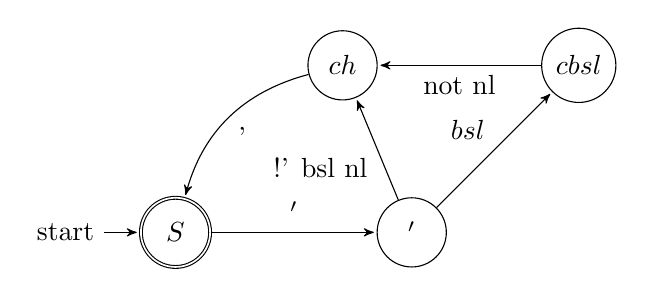
\begin{tikzpicture}[>=stealth',shorten >=1pt,auto,node distance=3cm]
	\node[initial,state,accepting](S) {$S$};
	\node[state] (') [right of=S] {$'$};
	\node[state] (cbsl) [above right of='] {$cbsl$};
	\node[state] (ch) [above right of=S] {$ch$};

	\path[->] (S) edge node {$'$} (')
	(') edge node {$bsl$} (cbsl)
	(') edge node {!' bsl nl} (ch)
	(cbsl) edge node {not nl} (ch)
	(ch) edge [bend right] node {'} (S)
	;
\end{tikzpicture}

\subsection{string literal}

"([!"\verb|\\|\verb|\|n]*|\verb|\|[!\verb|\|n])*"

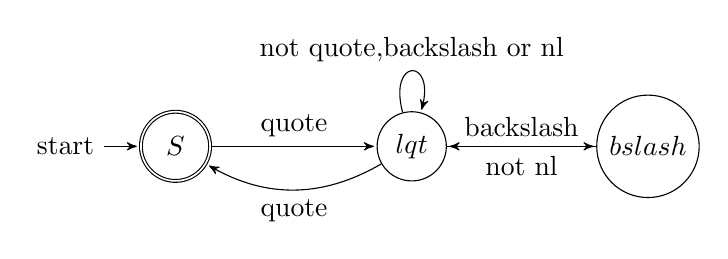
\begin{tikzpicture}[>=stealth',shorten >=1pt,auto,node distance=3cm]
	\node[initial,state,accepting](S) {$S$};
	\node[state] (lqt) [right of=S] {$lqt$};
	\node[state] (bslash) [right of=lqt] {$bslash$};

	\path[->] (S) edge node {quote} (lqt)
	(lqt) edge [loop above] node {not quote,backslash or nl} (lqt)
	(lqt) edge node {backslash} (bslash)
	(lqt) edge [bend left] node {quote} (S)
	(bslash) edge node {not nl} (lqt)
	;
\end{tikzpicture}

\subsection{comment}
(//[!\verb|\|]*) | (/\verb|\|*.*\verb|\|*/)

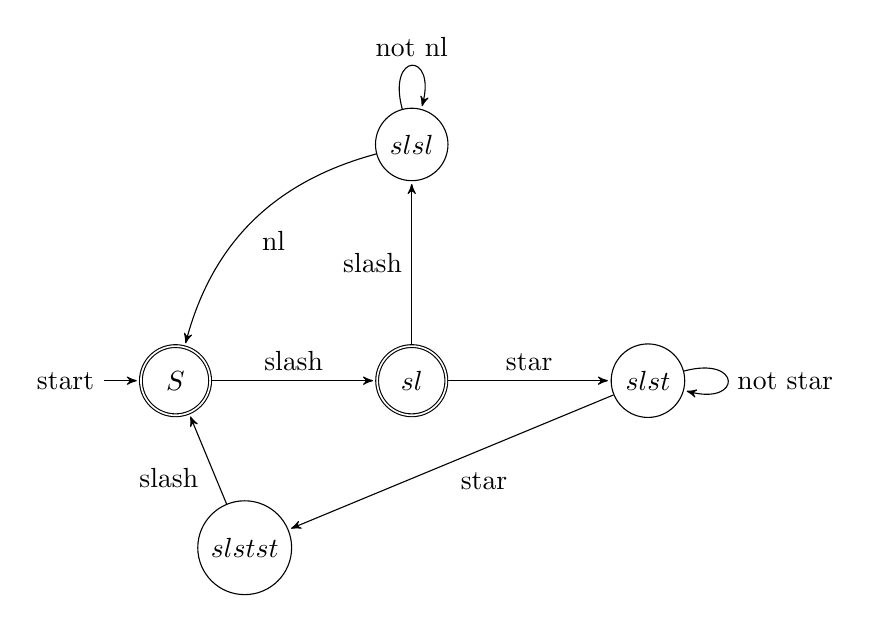
\begin{tikzpicture}[>=stealth',shorten >=1pt,auto,node distance=3cm]
	\node[initial,state,accepting](S) {$S$};
	\node[state,accepting] (sl) [right of=S] {$sl$};
	\node[state] (slst) [right of=sl] {$slst$};
	\node[state] (slstst) [below left of=sl] {$slstst$};
	\node[state] (slsl) [above of=sl] {$slsl$};

	\path[->] (S) edge node {slash} (sl)
	(sl) edge node {star} (slst)
	(sl) edge node {slash} (slsl)
	(slst) edge node {star} (slstst)
	(slst) edge [loop right] node {not star} (slst)
	(slstst) edge node {slash} (S)
	(slsl) edge [loop above] node {not nl} (slsl)
	(slsl) edge [bend right] node {nl} (S)
	;
\end{tikzpicture}

\subsection{identifier or keywords}
[A-Za-z\_][0-9A-Za-z\_]*

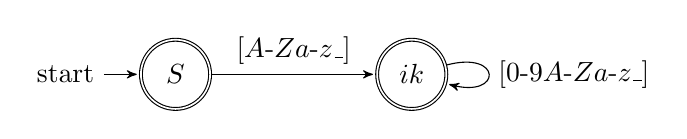
\begin{tikzpicture}[>=stealth',shorten >=1pt,auto,node distance=3cm]
	\node[initial,state,accepting](S) {$S$};
	\node[state, accepting](ik) [right of=S] {$ik$};
	
	\path[->] (S) edge node {$[A$-$Za$-$z\_]$} (ik)
	(ik) edge [loop right] node {$[0$-$9A$-$Za$-$z\_]$} (ik)
	;
\end{tikzpicture}

\section{automaton behavior}

\begin{enumerate}
	\item 
	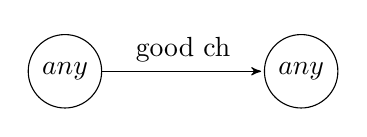
\begin{tikzpicture}[>=stealth',shorten >=1pt,auto,node distance=3cm]
		\node[state] (s) {$any$};
		\node[state] (s1) [right of=s] {$any$};
		\path[->] (s) edge node {good ch} (s1);
	\end{tikzpicture}
	\\move on
	\item 
	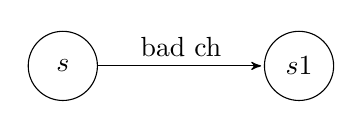
\begin{tikzpicture}[>=stealth',shorten >=1pt,auto,node distance=3cm]
		\node[state] (s) {$s$};
		\node[state] (s1) [right of=s] {$s1$};
		\path[->] (s) edge node {bad ch} (s1);
	\end{tikzpicture}
	\\report error
	\item 
	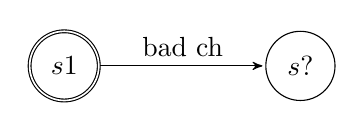
\begin{tikzpicture}[>=stealth',shorten >=1pt,auto,node distance=3cm]
		\node[state] (s) {$s?$};
		\node[state,accepting] (s1) [left of=s] {$s1$};
		\path[->] (s1) edge node {bad ch} (s);
	\end{tikzpicture}
	\\push back the character, parse the previous token, and return to initial state
	\item 
	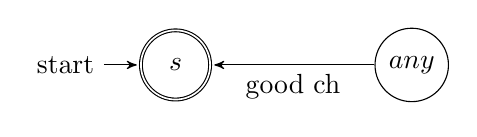
\begin{tikzpicture}[>=stealth',shorten >=1pt,auto,node distance=3cm]
		\node[state,initial,accepting] (s) {$s$};
		\node[state] (s1) [right of=s] {$any$};
		\path[->] (s1) edge node {good ch} (s);
	\end{tikzpicture}
	\\parse the token
\end{enumerate}

\end{document}